\documentclass[tikz]{standalone}
\begin{document}
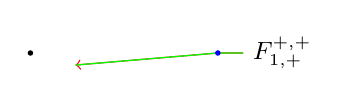
\begin{tikzpicture}[
  x={(1.10cm,-0.55cm)},
  y={(-1.10cm,-0.55cm)},
  z={(0cm,1.18cm)},
  font=\small]
  \coordinate (qf representative) at (1,0.48,0.56);
  \begin{scope}[x=1cm,y=1cm]
    \fill[black] (0,0) circle (1pt);
    \node[anchor=west] (qf label) at (2.70,0.00) {$F_{1,+}^{+,+}$};
    \draw[red,->,line width=0.45pt] (qf label.west)--(2.38,0.00)--(qf representative);
    \draw[green,line width=0.45pt] (qf label.west)--(2.38,0.00)--(qf representative);
    \fill[blue] (2.38,0) circle (1pt);
  \end{scope}
\end{tikzpicture}
\end{document}
